La interacción entre los distintos servicios que se desarrollan en este proyecto se realizarán mediante una \gls{API}(Application Programming Interface). Entre los dos paradígmas más utilizados a la hora de crear APIs se encuentran RPC y REST. Se va a escoger el estandar RPC por responder a los requisistos a los que nos enfrentamos.

\textbf{GRPC}

Según el paper original que describe el paradígma RPC “Remote procedure calls (RPC) appear to be a useful paradigm for providing communication across a
network between programs written in a high-level language.“~\cite{Birrell198439}. RPC permite ejecutar una llamada a un servicio en un servidor remoto mediante formularios predefinidos, obteniendo respuestas con el mismo formato. El estilo del servidor que realiza la llamada, no se tiene en cuenta por diseño. Lo cual permite abstraernos de la implementación.

gRPC (Google Remote Procedure Call~\cite{grpc}) es un subtipo del diseño RPC.  es una arquitectura global de alto rendimiento y de código abierto que garantiza la flexibilidad y la velocidad de la arquitectura de microservicios. Se dispone de un \gls{IDL} (interface definition language) empleando Protocol Buffers para definir la interfaz del servicio y el formato de los mensajes de carga útil. Suministra un mecanismo para traducirlo a diversos lenguajes de desarrollo. Con un único lenguaje obtenemos la capacidad de describir interfaces sin implicarnos en la implementación.

RPC utiliza el estándar HTTP 2.0, pero ni el servidor ni el programador de la API tienen conocimiento de HTTP. Como resultado, la complejidad disminuye porque no hay que preocuparse por cómo se traducen los principios de RPC a HTTP. gRPC acelera la transferencia de datos entre microservicios, tanto en tiempo de desarrollo como de ejecución.

\textbf{REST}

\gls{REST} (Representational State Transfer) es un paradigma cliente-servidor de comunicación donde se comunican a través de mensajes codificados en formato JSON o XML o compatibles. En su disertación original del año 2000, Roy T. Fielding define la interaccion REST como: “The a server will respond with the representation of a resource (today, it will most often be an HTML, XML or JSON document) and that resource will contain hypermedia links that can be followed to make the state of the system change. Any such request will in turn receive the representation of a resource, and so on.“ ~\cite{FieldingRoyThomas2000Asat}. En la misma disertación enumera los principios que ha de seguir el estandar:

\begin{itemize}
    \item Arquitectura cliente-servidor. Hace hincapié en la separación de responsabilidades
    \item Ausencia de estado. El estado se guarda y mantiene en el cliente y no en el servidor
    \item Todas las solicitudes deben declarar si son o no cacheables
    \item Interfaz unifome
    \item Sistema por capas. Tiene relación con la separación de responsabilidades
\end{itemize}

Cada componente que combina el sistema de microservicios puede mostrarse y hacerse accesible públicamente al usuario o al cliente como un recurso de la API REST. Este recurso puede consultarse mediante los comandos HTTP GET, POST, PUT y DELETE. el usuario envía una consulta a una URL (Uniform Resource Locator) que provoca una respuesta con una carga útil en JSON, XML o cualquier formato de datos compatible. Esta carga útil representa el recurso que desea el usuario. Las peticiones comunes de los clientes incluyen:

\begin{itemize}
    \item Un método HTTP que especifica lo que debe procesarse en el recurso
    \item La ruta del recurso
    \item La cabecera que contiene datos sobre la consulta
    \item Una carga útil de mensaje específica del cliente
\end{itemize}

El servidor de la API envía una cabecera de tipo de contenido que identifica el formato de entrega del mensaje empleado en el cuerpo de la respuesta junto con la carga útil de datos que entrega al usuario que realiza la consulta. También se incluye en el cuerpo de la respuesta un código de respuesta que informa al usuario del estado del resultado de la llamada a la API.

\textbf{HTTP 1.1 frente a HTTP 2}

El protocolo HTTP/2 para transmitir mensajes permite flujos multiplexados y una comunicación bidireccional. gRPC admite varios tipos de interacciones, incluyendo interacciones unarias, streaming de servidor, streaming de cliente y streaming bidireccional. En contraste, REST utiliza el modelo de petición-respuesta de HTTP 1.1 que utiliza un método de handshaking TCP para cada consulta, lo que puede causar problemas de latencia y no aprovechar las ventajas de HTTP/2. En general, gRPC puede proporcionar una transmisión de datos más rápida y eficiente y una comunicación más flexible y bidireccional en comparación con REST.

\textbf{La estructura de datos de la carga útil}

gRPC utiliza Protocol Buffers para serializar y deserializar datos, lo que permite una transmisión más rápida y eficiente de información. Este método es más ligero, ya que los mensajes son una estructura más comprimida. Están en formato binario, lo que hace que el procesamiento sea menos intensivo en CPU. En el intercambio de datos, serializa y deserializa la información de forma automática.

REST utiliza principalmente JSON o XML para enviar y recibir información. La facilidad de lectura humana de JSON es una ventaja de REST, pero no es tan rápido o ligero. Esto se debe al requerimiento de que JSON debe ser serializado y traducido a los lenguajes de programación utilizados en ambos extremos. Este paso adicional en el proceso de transmisión de datos puede afectar la eficiencia y aumentar la probabilidad de errores.


\textbf{Compatibilidad con los navegadores}\label{GRPCcompatibilidadConNavegadores}

Dado que la mayor parte de la interacción de la API web se produce en línea, la compatibilidad con el navegador es una consideración clave en el debate entre gRPC vs. REST. La compatibilidad con los navegadores es probablemente una de las principales ventajas de las APIs REST frente a gRPC. Todos los navegadores ofrecen compatibilidad completa con HTTP 1.1. Sin embargo, la compatibilidad HTTP.2 para gRPC los navegadores sigue siendo relativamente restringida. En la web se necesita traducir la comunicacion  HTTP 2 a HTTP 1.1. por lo se hace necesario establecer una capa proxy; añadiendo un elemento de complejidad y mantenimiento. El soporte de HTTP 2 para los navegadores es algo que se encuentra todavía en desarrollo.

\textbf{Generación de código}

Para el IDL de gRPC existe un compilador llamado protoc que carga los archivos con la extensión de dicho lenguaje (.proto) y genera código nativo para comunicarse con los servicios remotos. Están soportados múltiples lenguajes de programación. En REST se debe emplear herramientas de terceros, como Postman, para la generación de código para las consultas de la API. La generación automática del código para la comunicación es especialmente ventajosa para los microservicios que combinan múltiples plataformas y lenguajes. Facilita la construcción del kit de desarrollo de software (SDK) para cada lenguaje y facilita enfrentar cambios en la interfaz.

\textbf{Justificación de uso de gRPC}

Aunque actualmente la mayoría de las herramientas de terceros no ofrecen soporte gRPC, es una tecnología adecuada para la interacción entre sistemas internos, como microservicios. Además, permite la interoperabilidad entre distintos lenguajes de programación, lo cual es otro de sus puntos fuertes. Otro beneficio del uso de gRPC es la transmisión en stream de información sin necesidad de reestablecer la comunicación para el envío de cada paquete de datos, lo cual es crítico si se quiere trabajar en sistemas que enfrenten el tiempo real. El control de dispositivos mediante sistemas PID hace que esta característica sea esencial. Las conexiones tanto de streaming, por parte del cliente como del servidor, permite establecer canales de comunicación versátiles según la situación a la que nos enfrentemos. La monitorización de los dispositivos controlados, necesitamos una optimización en el uso del ancho de banda. Aquí es donde gRPC sobresale, ya que proporciona una comunicación ligera, mayor eficiencia y rapidez. En la figura~\cref{fig:gRPC vs REST} se resume la comparación entre los dos sistemas.

\begin{figure}[H]
    \centering
    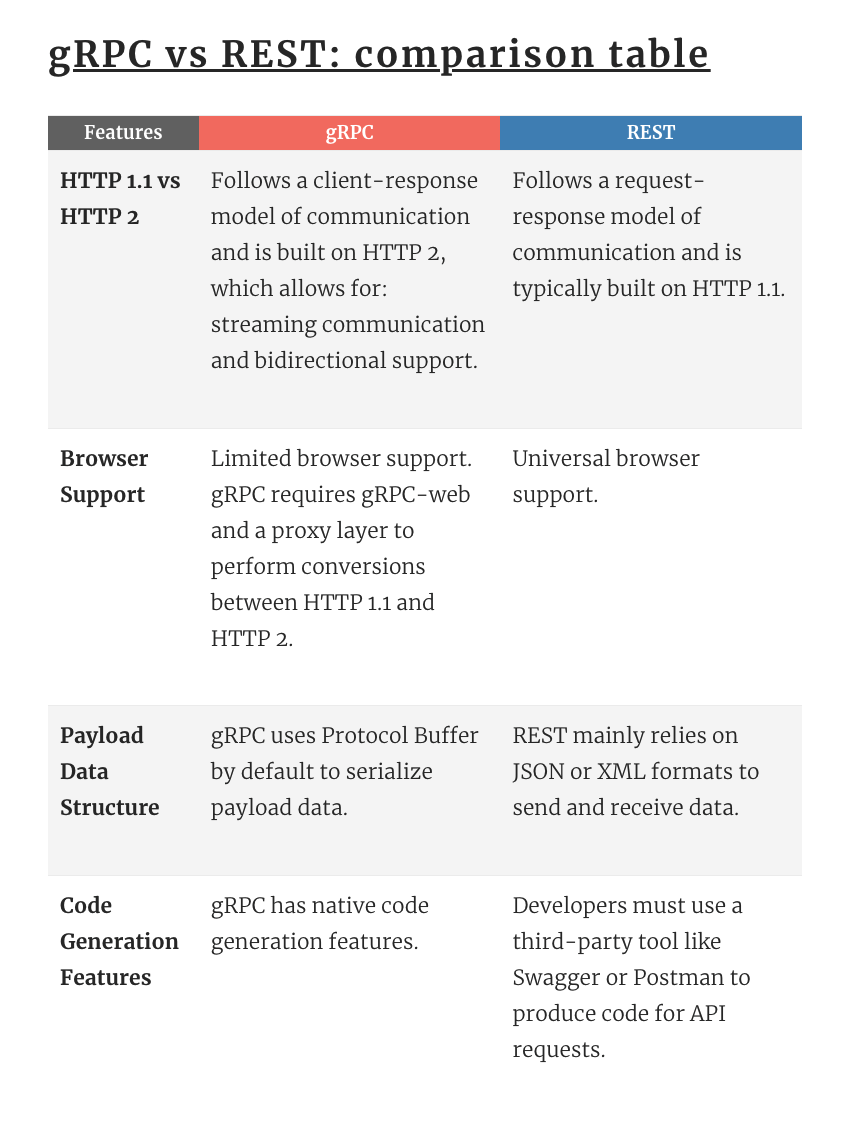
\includegraphics[height=0.4\textheight]{./part/Proyecto_ejecutivo/memoria_constructiva/rpc/img/rpcComparison}
    \caption{gRPC vs REST.\cite{berga_santos_2023}}\label{fig:gRPC vs REST}
\end{figure}